
%%%%%%%%%%%%%%%%%%%%%%%%%%%%%%%%%%%%%%%%%%%%%%%%%%%%%%%%
%
% Copyright (c) 2003-2009 by University of Queensland
% Earth Systems Science Computational Center (ESSCC)
% http://www.uq.edu.au/esscc
%
% Primary Business: Queensland, Australia
% Licensed under the Open Software License version 3.0
% http://www.opensource.org/licenses/osl-3.0.php
%
%%%%%%%%%%%%%%%%%%%%%%%%%%%%%%%%%%%%%%%%%%%%%%%%%%%%%%%%

\section{Two Dimensional Heat Diffusion for a basic Magmatic Intrusion}
%\label{Sec:2DHD}
 Building upon our success from the 1D models it is now prudent to expand our domain by another dimension. For this example we will be using a very simple magmatic intrusion as the basis for our model. The simulation will be a single event where some molten granite has formed a hemisphericle dome at the base of some cold sandstone country rock. A hemisphere is semetric so taking a cross-section through its centre will effectively model a 3D problem in 2D. New concepts will include non-linear boundaries and the abilitity to prescribe location specific variables.

\begin{figure}[h!]
\centerline{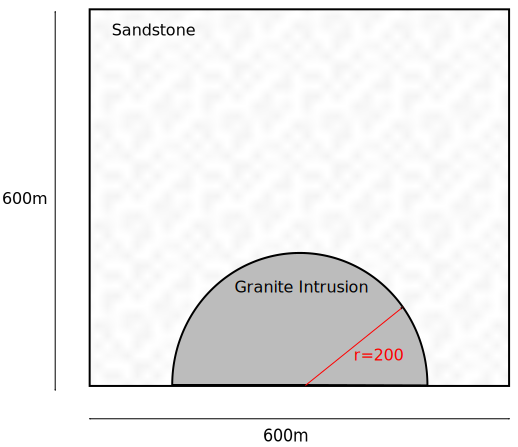
\includegraphics[width=4.in]{figures/twodheatdiff}}
\caption{2D model: granitic intrusion of sandstone country rock.}
\label{fig:twodhdmodel}
\end{figure}

To expand upon our 1D problem, the domain must first be expanded. This will be done in our definition phase by creating a square domain in $x$ and $y$ that is 600 meters along eacy side \reffig{fig:twodhdmodel}. The number of discrete spatial cells will be 100. The radius of the intrusion will be 200 meters  And the location of the centre of the intrusion will be at the 300 meter mark on the x-axis. The domain variables are;
\begin{verbatim}
mx = 600 # model lenght
my = 600 # model width
ndx = 100 # steps in x direction 
ndy = 100 # steps in y direction
r = 200 # radius of intrusion
ic = [300, 0] #centre of intrusion 
\end{verbatim}
The next step is to define our variables for each material in the model in a manner similar to the previous tutorial. Note that each material has its own unique set of values. The time steps and set up for the domain remain as before. Prior to setting up the PDE the boundary between the two materials must be established. The distance $s$ between two points in car cartesian coordinates is defined as:
\begin{equation}
 (x_{1}-x_{0})^{2}+(y_{1}-y_{0})^{2} = s^{2}
\end{equation}
If $[x_{0},y_{0}]$ is the point $c$ the centre of the semi-circle that defines our intrusion then for all the points $[x,y]$ in our solution space we can define a distance to $c$. Hence, and points that fall within the radius $r$ of our intrusion will have a coresponding value $s < r$ and all those belonging to the country rock will have a value $s > r$. By subtracting $r$ from both of these conditions we find $s-r < 0$ for all intrusion points and $s-r > 0$ for all country rock points. Defining these conditions into the code is quite simple and is done using the following command:
\begin{verbatim}
 bound = length(x-ic)-r #where the boundary will be located
\end{verbatim}
This definition of the boundary can now be used with the \verb wherePositive()  and \verb whereNegative()  commands from before to help define the material constants and temperatures in our domain. By examining the general form we solved in the earlier tutorials, it is obvious that both \verb A  and \verb D  depend on the predefined variables. To set these variables accordingly and complete our PDE we use:
\begin{verbatim}
A = (kappai)*whereNegative(bound)+(kappac)*wherePositive(bound)
D = (rhocpi/h)*whereNegative(bound)+(rhocpc/h)*wherePositive(bound)

mypde.setValue(A=A*kronecker(model),D=D,d=eta,y=eta*Tc)
\end{verbatim}
Our PDE has now been properly established. The initial conditions for temperature are set out in a similar matter:
\begin{verbatim}
 T= Ti*whereNegative(bound)+Tc*wherePositive(bound) #defining the initial temperatures.
\end{verbatim}
The itteration process now begins as before, but using our new conditions for \verb D  as defined above.

\subsection{Contouring escript data}
\begin{verbatim}
# rearrage mymesh to suit solution function space      
oldspacecoords=model.getX()
coords=Data(oldspacecoords, T.getFunctionSpace())
coords = np.array(coords.toListOfTuples())
coordX = coords[:,0]
coordY = coords[:,1]
# create regular grid
xi = np.linspace(0.0,600.0,100)
yi = np.linspace(0.0,600.0,100)
\end{verbatim}

